\problemname{Losing Leaves}

%\illustration{0.3}{image.jpg}{
%    Caption of the illustration (optional).
%    CC BY-SA 4.0 by X on \href{https://example.com/reference-to-image}{Y}
%}

% optionally define variables/limits for this problem
\newcommand{\maxn}{10^6}

Here at the Benelux Advanced Phone Company (BAPC),
we are the proud owners of the largest telephone network in the Benelux area.
Unfortunately, our network has become too large for us to manage properly.
As such, we have decided to sell part of our network.

\begin{wrapfigure}{r}{0.3\textwidth}
    \centering
    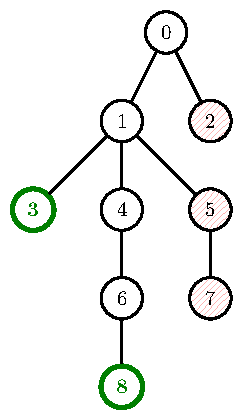
\includegraphics{figure.pdf}
    \caption{
        Visualization of the second sample input.
    }
    \label{fig:leaves}
\end{wrapfigure}

The network of the BAPC consists of interconnected transmission nodes.
One transmission node is marked as the central switch.
All other nodes have exactly one upstream transmission node.
For each transmission node, if we follow the upstream connections, we will finally end up at the central switch.
A node is considered a customer transmission node when it is a leaf,~i.e.~when it has no downstream nodes.

When selling parts of our network, integrity must be maintained.
That means that whenever we sell a transmission node $X$, we also have to sell
nodes downstream of $X$.

Overall, BAPC decided to sell exactly $k$ transmission nodes.
While there may be many options to choose these $k$ nodes, we actually want to make our lives as easy as possible:
After selling, we want to minimize the number of customer transmission nodes in our network, while maintaining the network's integrity.

As an example, consider the second sample case, visualized in Figure~\ref{fig:leaves}.
The three striped red nodes are sold, and the two bold green nodes are the remaining customer nodes.

\begin{Input}
    The input consists of:
    \begin{itemize}
        \item One line with two integers $n$ and $k$ ($0\leq k < n\leq \maxn$), the number of transmission nodes, and the number of nodes to sell.
        \item
            $n-1$ lines, the \(i\)th of which contains one integer \(p_i\) (\(0 \leq p_i < i\))
            indicating that transmission node \(i\) (\(1 \leq i < n\)) has an outgoing connection to node \(p_i\).
    \end{itemize}

    The transmission nodes are numbered from \(0\) to \(n - 1\), inclusive.
    Node $0$ is always the central switch.
\end{Input}

\begin{Output}
    Output the minimum number of customer transmission nodes after selling $k$ transmission nodes.
    Note that if the central switch is the only remaining node, it also counts as a customer node.
\end{Output}
